\documentclass{beamer}

\usepackage[utf8]{inputenc}
\usepackage{hyperref}

\usetheme{Berkeley}
\beamertemplatenavigationsymbolsempty
\setbeamertemplate{headline}{}
 
\title{Erfassen von Daten in FoodChain-Lab 2}
\date{}
 
\begin{document}
\maketitle

\section{ }

\subsection{Aufgaben}
\begin{frame}
	\begin{itemize}
		\item
	\end{itemize}
\end{frame}
 
\subsection{1}
\begin{frame}
	\begin{center}
  		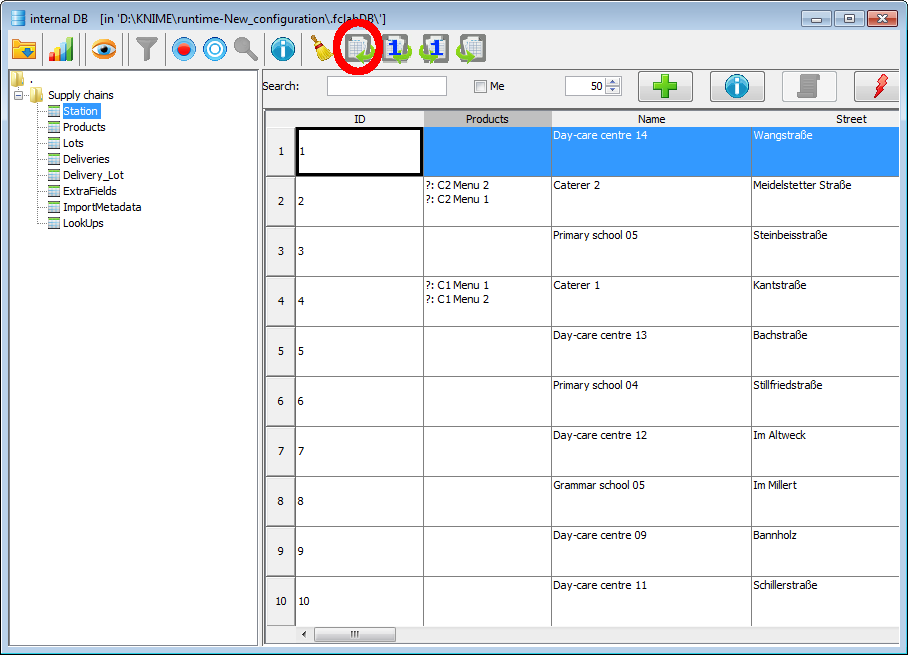
\includegraphics[height=0.6\textheight]{1.png}
	\end{center}
	\begin{itemize}
		\item Wählen Sie \textbf{Food-Lab $>$ Open DB Gui...} in der Menüleiste um das Datenbank-Fenster zu öffnen.
	\end{itemize}
\end{frame}

\subsection{2}
\begin{frame}
	\begin{center}
  		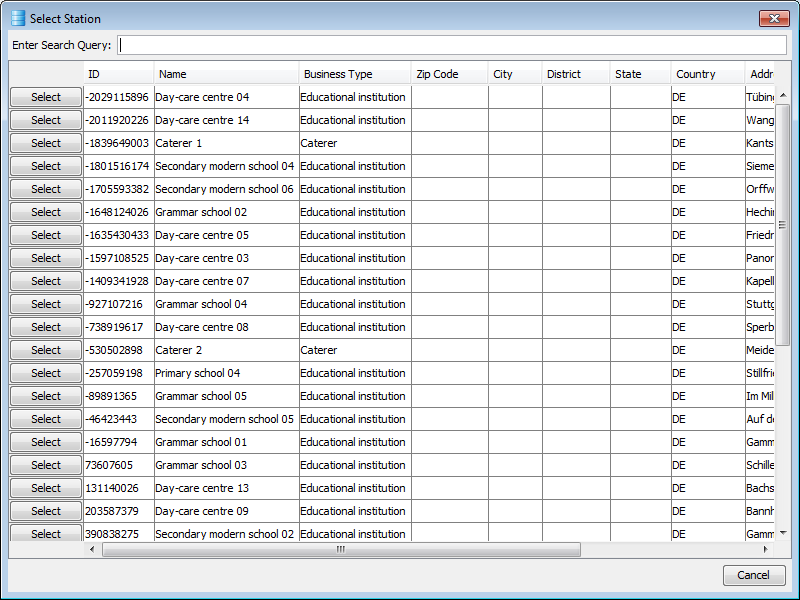
\includegraphics[width=0.4\textwidth]{2.png}
	\end{center}
	\begin{itemize}
		\item
	\end{itemize}
\end{frame}

\subsection{3}
\begin{frame}
	\begin{center}
  		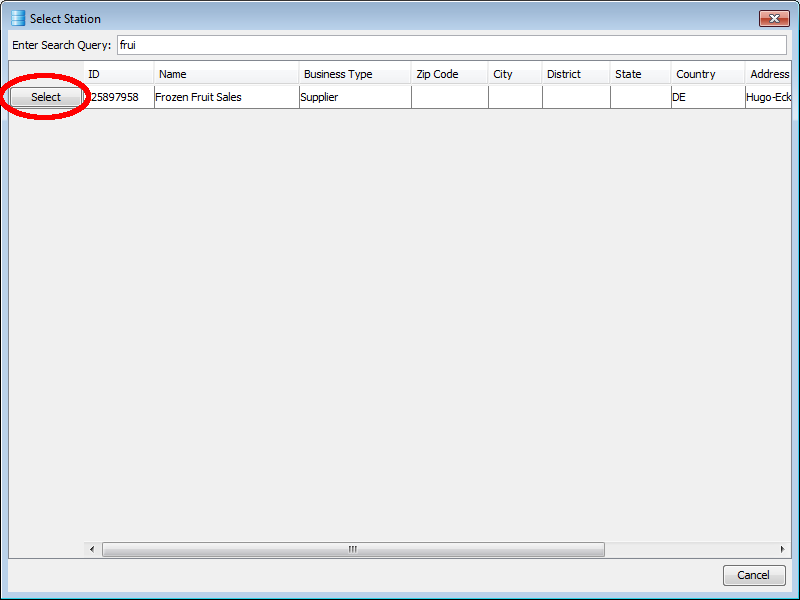
\includegraphics[height=0.5\textheight]{3.png}
	\end{center}
	\begin{itemize}
		\item
	\end{itemize}
\end{frame}

\subsection{4}
\begin{frame}
	\begin{center}
  		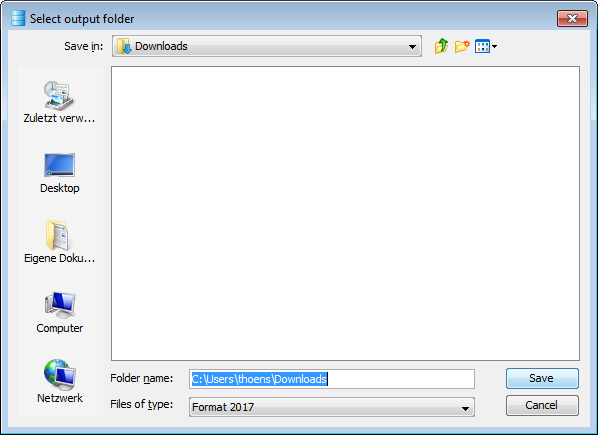
\includegraphics[width=0.8\textwidth]{4.png}
	\end{center}
	\begin{itemize}
		\item
	\end{itemize}
\end{frame}

\subsection{5}
\begin{frame}
	\begin{center}
  		
\includegraphics[width=0.95\textwidth]{5.png}
	\end{center}
	\begin{itemize}
		\item
	\end{itemize}
\end{frame}

\subsection{6}
\begin{frame}
	\begin{center}
  		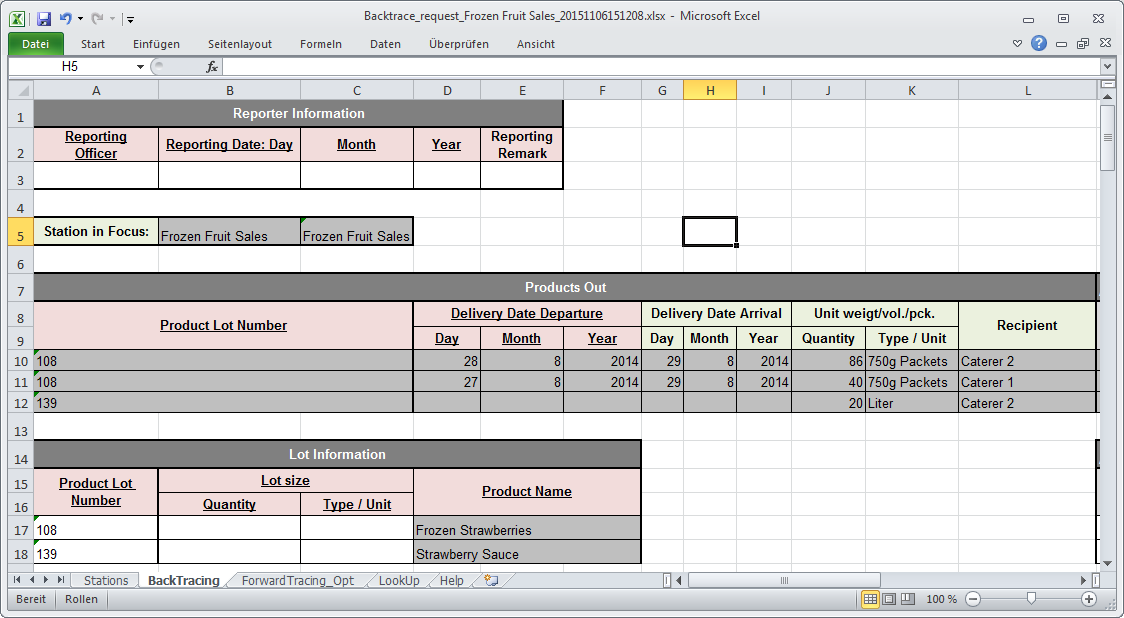
\includegraphics[width=0.95\textwidth]{6.png}
	\end{center}
	\begin{itemize}
		\item
	\end{itemize}
\end{frame}

\subsection{7}
\begin{frame}
	\begin{center}
  		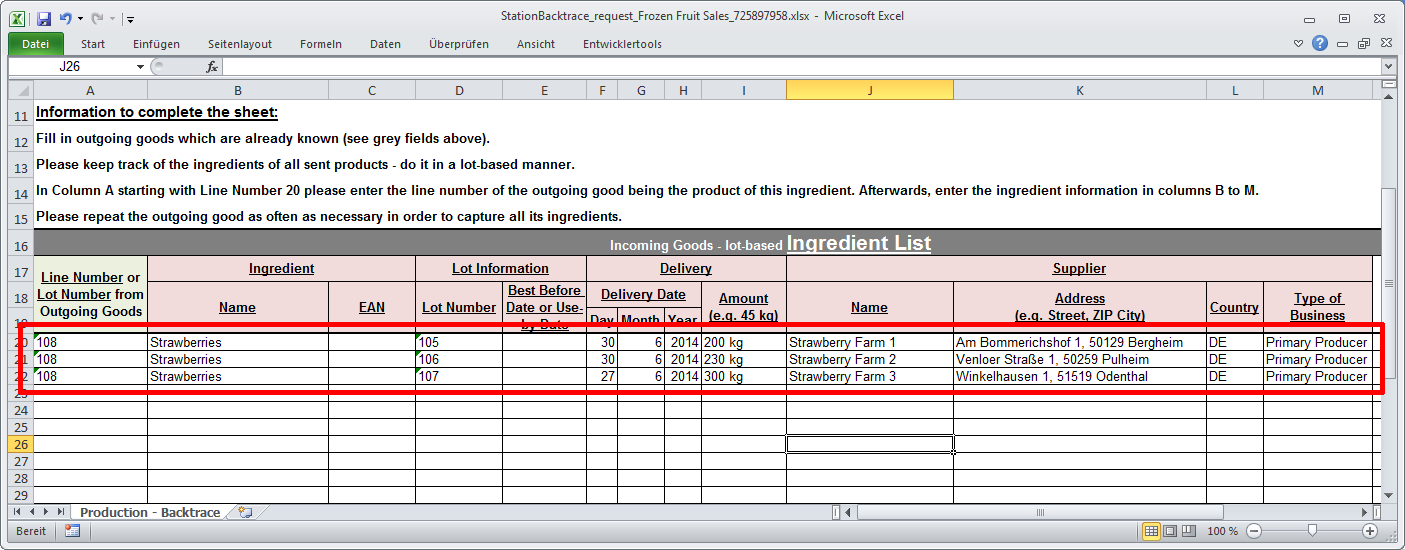
\includegraphics[width=0.95\textwidth]{7.png}
	\end{center}
	\begin{itemize}
		\item
	\end{itemize}
\end{frame}

\subsection{8}
\begin{frame}
	\begin{center}
  		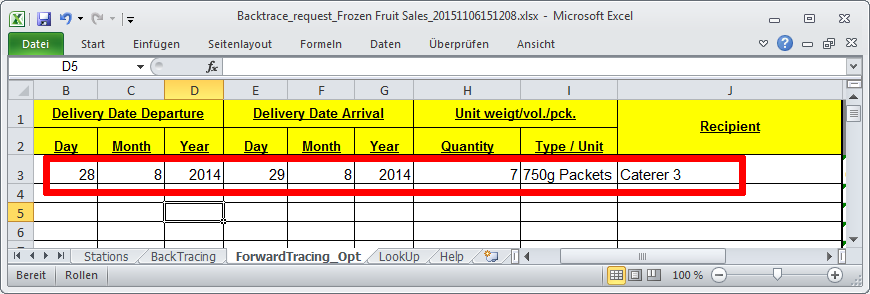
\includegraphics[width=0.95\textwidth]{8.png}
	\end{center}
	\begin{itemize}
		\item
	\end{itemize}
\end{frame}

\subsection{9}
\begin{frame}
	\begin{center}
  		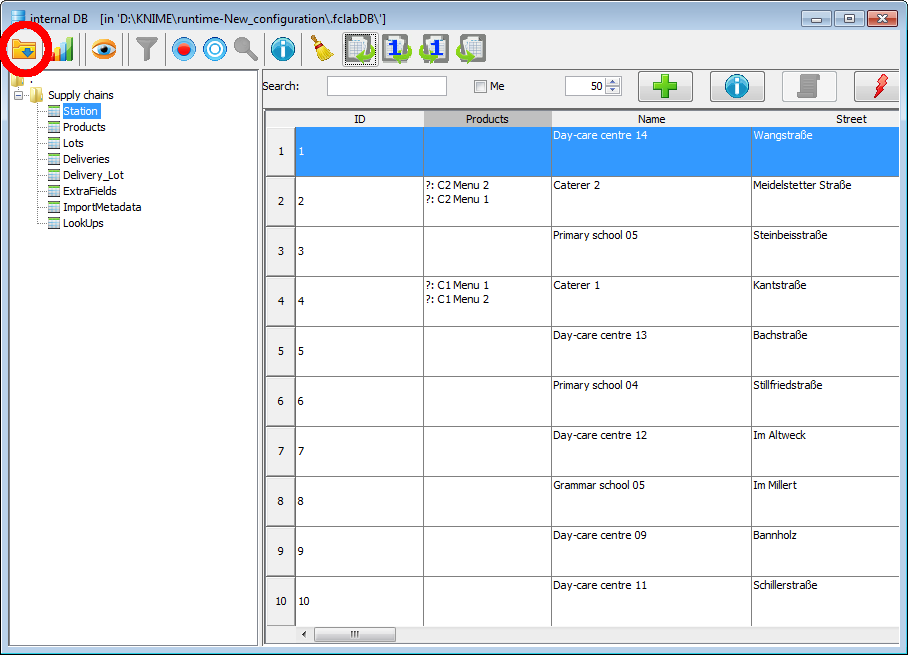
\includegraphics[height=0.6\textheight]{9.png}
	\end{center}
	\begin{itemize}
		\item
	\end{itemize}
\end{frame}

\subsection{10}
\begin{frame}
	\begin{center}
  		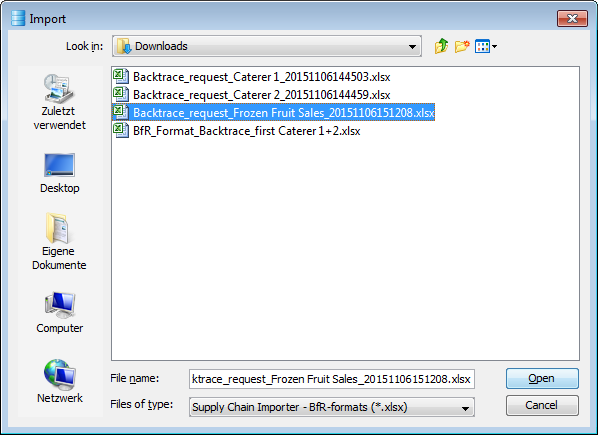
\includegraphics[height=0.5\textheight]{10.png}
	\end{center}
	\begin{itemize}
		\item
	\end{itemize}
\end{frame}

\subsection{11}
\begin{frame}
	\begin{center}
  		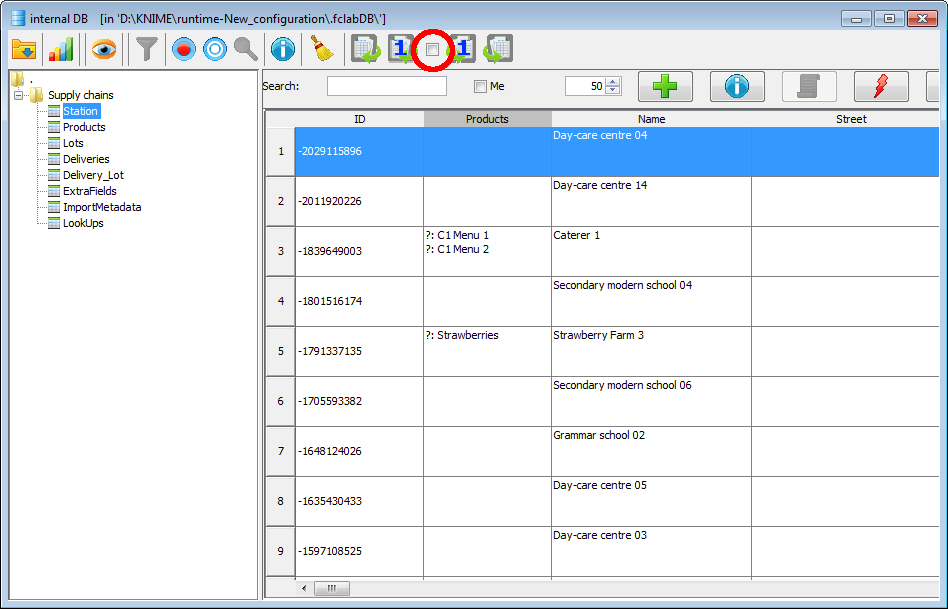
\includegraphics[width=0.7\textwidth]{11.png}
	\end{center}
	\begin{itemize}
		\item
	\end{itemize}
\end{frame}

\subsection{12}
\begin{frame}
	\begin{center}
  		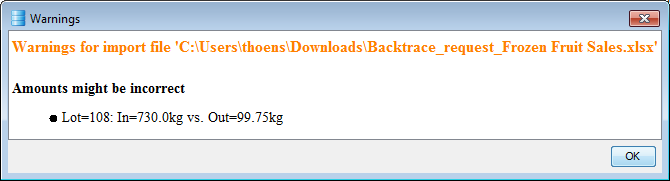
\includegraphics[width=0.95\textwidth]{12.png}
	\end{center}
	\begin{itemize}
		\item
	\end{itemize}
\end{frame}

\subsection{13}
\begin{frame}
	\begin{center}
  		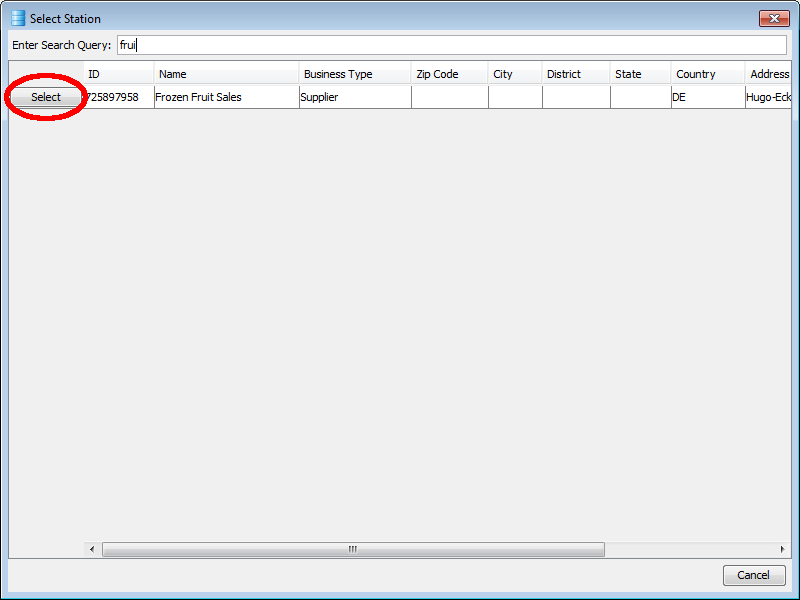
\includegraphics[height=0.6\textheight]{13.png}
	\end{center}
	\begin{itemize}
		\item
	\end{itemize}
\end{frame}

\subsection{14}
\begin{frame}
	\begin{center}
  		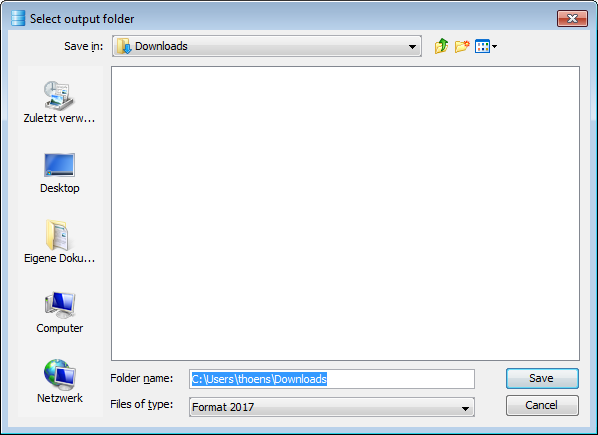
\includegraphics[width=0.95\textwidth]{14.png}
	\end{center}
	\begin{itemize}
		\item
	\end{itemize}
\end{frame}

\subsection{15}
\begin{frame}
	\begin{center}
  		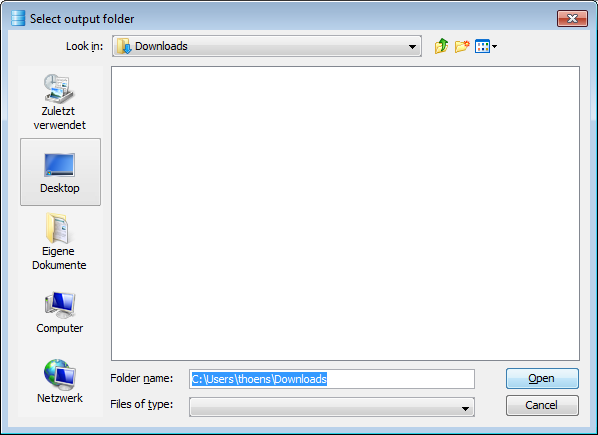
\includegraphics[height=0.5\textheight]{15.png}
	\end{center}
	\begin{itemize}
		\item
	\end{itemize}
\end{frame}

\subsection{16}
\begin{frame}
	\begin{center}
  		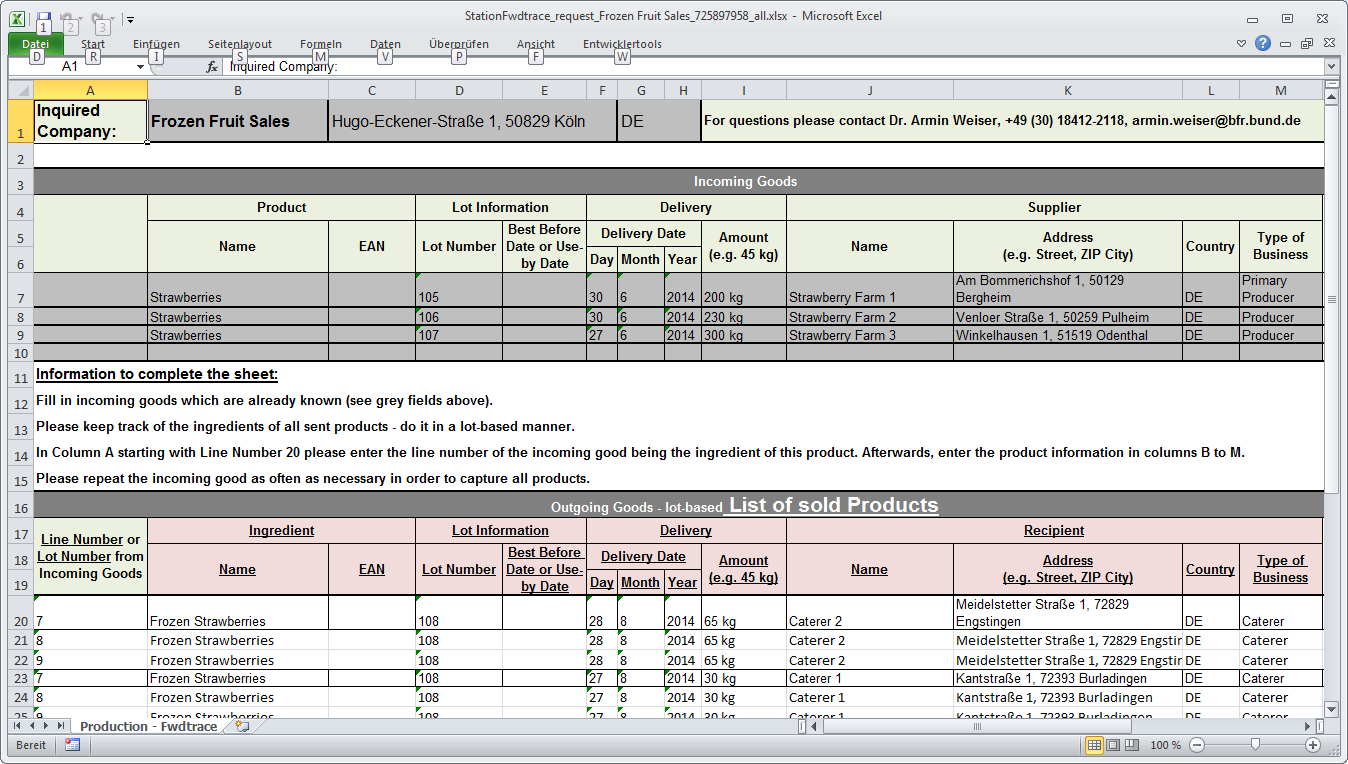
\includegraphics[width=0.8\textwidth]{16.png}
	\end{center}
	\begin{itemize}
		\item
	\end{itemize}
\end{frame}

\subsection{17}
\begin{frame}
	\begin{center}
  		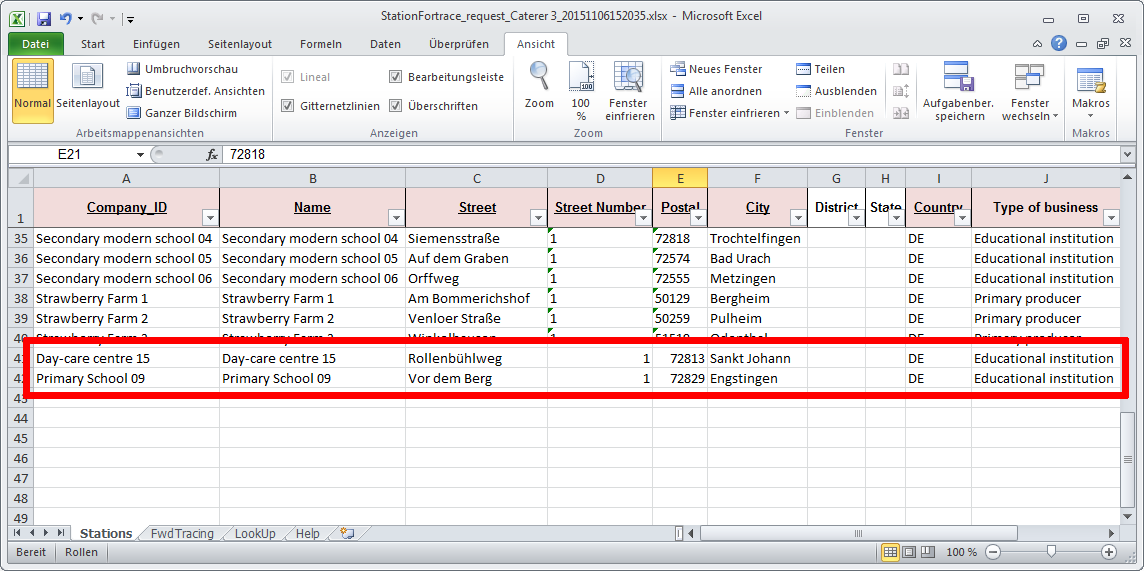
\includegraphics[width=0.95\textwidth]{17.png}
	\end{center}
	\begin{itemize}
		\item
	\end{itemize}
\end{frame}

\subsection{18}
\begin{frame}
	\begin{center}
  		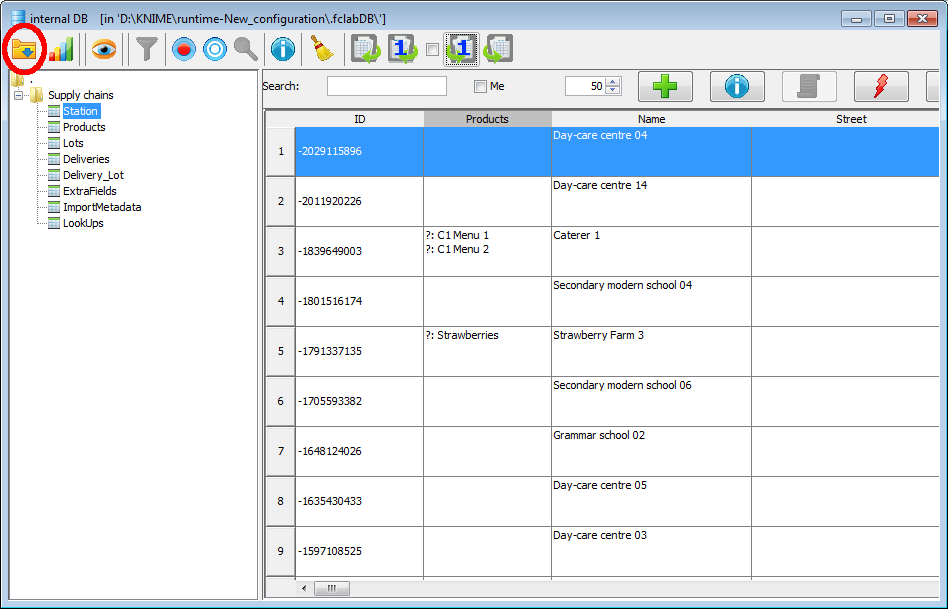
\includegraphics[width=0.95\textwidth]{18.png}
	\end{center}
	\begin{itemize}
		\item
	\end{itemize}
\end{frame}

\subsection{19}
\begin{frame}
	\begin{center}
  		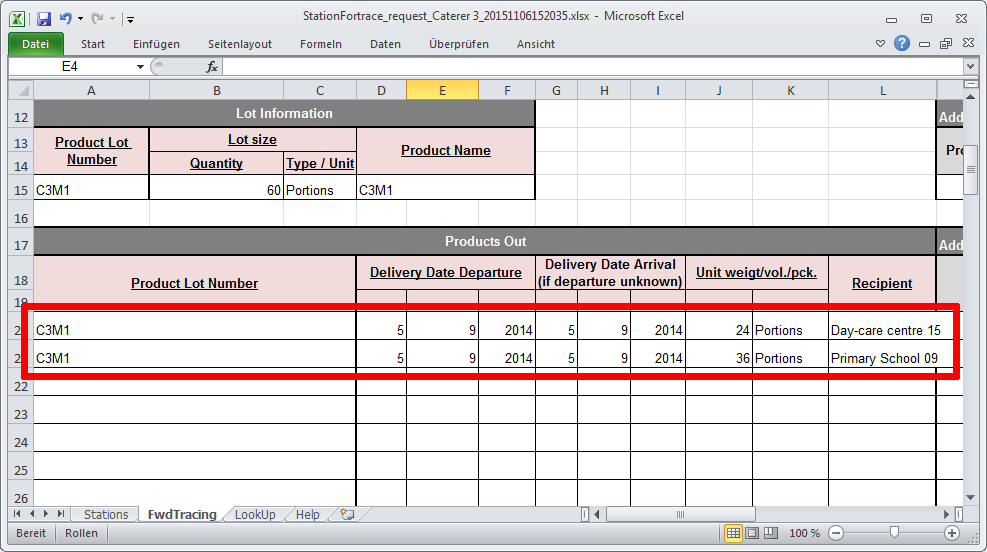
\includegraphics[width=0.95\textwidth]{19.png}
	\end{center}
	\begin{itemize}
		\item
	\end{itemize}
\end{frame}

\subsection{20}
\begin{frame}
	\begin{center}
  		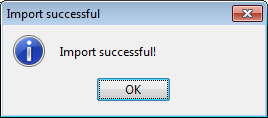
\includegraphics[height=0.6\textheight]{20.png}
	\end{center}
	\begin{itemize}
		\item
	\end{itemize}
\end{frame}

\subsection{21}
\begin{frame}
	\begin{center}
  		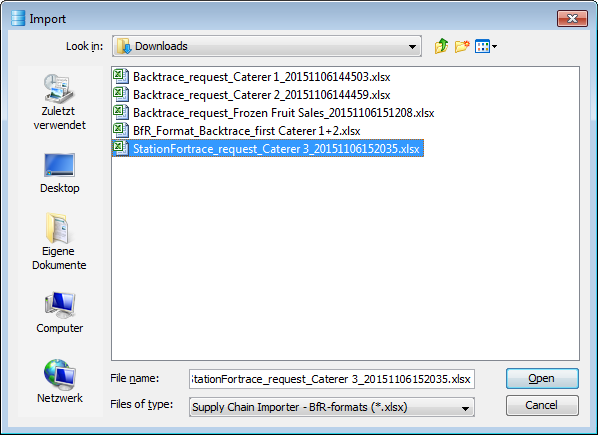
\includegraphics[height=0.5\textheight]{21.png}
	\end{center}
	\begin{itemize}
		\item
	\end{itemize}
\end{frame}

\subsection{22}
\begin{frame}
	\begin{center}
  		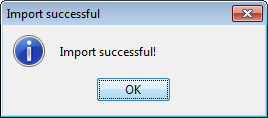
\includegraphics[width=0.4\textwidth]{22.png}
	\end{center}
	\begin{itemize}
		\item
	\end{itemize}
\end{frame}

\end{document}